\documentclass{article}

\usepackage{pandekten}
\usepackage{dashrule}

\makeatletter
\newcommand*{\shifttext}[1]{%
  \settowidth{\@tempdima}{#1}%
  \hspace{-\@tempdima}#1%
}
\newcommand{\plabel}[1]{%
\shifttext{\textbf{#1}\quad}%
}
\newcommand{\prule}{%
\begin{center}%
\hdashrule[0.5ex]{.99\linewidth}{1pt}{1pt 2.5pt}%
\end{center}%
}

\makeatother

\newcommand{\minusbaseline}{\abovedisplayskip=0pt\abovedisplayshortskip=0pt~\vspace*{-\baselineskip}}%

\setlength{\parindent}{0pt}

\title{Assignment 9}
\author{Ze Chen}

\begin{document}

\maketitle

\plabel{1 (a)}%
For $\lambda = 0$,
\[ H = \int \dd[3]{x} \sum_i \qty(\frac{1}{2} (\Pi^i)^2 + \frac{1}{2} (\grad \Phi^i)^2 + \frac{1}{2} m^2 (\Phi^i)^2), \]
which consists of $N$ independent real scalar fields, and therefore the propagators are just
\[ \wick{\c1 \Phi^i(x) \c1 \Phi^j(y)} = \delta^{ij} D_{\mathrm{F}}(x-y). \]
The vertex is given by
\begin{align*}
  &\phantom{{}={}} 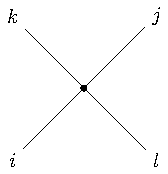
\includegraphics{img/phi4/phi4.pdf} \\
  &= -i\frac{\lambda}{4} \sum_p \sum_q \text{number of contractions of } \qty(\Phi^i \Phi^j \Phi^k \Phi^l \Phi^p \Phi^p \Phi^q \Phi^q) \\
  &= -i \frac{\lambda}{4} \sum_p \sum_q 4\big(
    \delta^{ip}\delta^{jp}\delta^{kq}\delta^{lq} + \delta^{ip}\delta^{kp}\delta^{jq}\delta^{lq} + \delta^{ip}\delta^{lp}\delta^{jq}\delta^{kq}\\
  &\phantom{-i \frac{\lambda}{4} \sum_p \sum_q 4\big(} + \delta^{jp}\delta^{kp}\delta^{iq}\delta^{lq} + \delta^{jp}\delta^{lp}\delta^{iq}\delta^{kq} + + \delta^{kp}\delta^{lp}\delta^{iq}\delta^{jq}\big) \\
  &= -2 i \lambda\qty(\delta^{ij}\delta^{kl} + \delta^{il}\delta^{jk} + \delta^{ik} \delta^{jl}).
\end{align*}
The differential cross section is given by
\[ \qty(\dv{\sigma}{\Omega})_{\mathrm{CM}} = \frac{\abs{\mathcal{M}}^2}{64\pi^2 E^2_{\mathrm{cm}}} \]
where
\begin{align*}
  \abs{\mathcal{M}(\Phi^1\Phi^2 \rightarrow \Phi^1\Phi^2)}^2 &= 4\lambda^2, \\
  \abs{\mathcal{M}(\Phi^1\Phi^1 \rightarrow \Phi^2\Phi^2)}^2 &= 4\lambda^2, \\
  \abs{\mathcal{M}(\Phi^1\Phi^1 \rightarrow \Phi^1\Phi^1)}^2 &= 36\lambda^2.
\end{align*}

\plabel{(b)}%
Since $v^2 = \mu^2 / \lambda$, the Lagrangian is given by (removing constant terms)
\begin{align*}
  \mathcal{L} &= \frac{1}{2}(\partial_\mu \sigma)^2 - \frac{1}{2}(2\mu^2)\sigma^2 + \qty(\frac{1}{2} \sum_k (\partial_\mu \pi^k)^2) \\
  &\phantom{{}={}} - \sqrt{\lambda}\mu\sigma^3 - \qty(\sum_k \sqrt{\lambda}\mu\sigma (\pi^k)^2) - \frac{\lambda}{4}\sigma^4 - \qty(\sum_k \frac{\lambda}{2} \sigma^2 (\pi^k)^2) - \qty(\sum_k \frac{\lambda}{4}(\pi^k)^2)^2.
\end{align*}
The Feynman rules are listed below (colored line for $\sigma$ and black line for $\pi^i$).
\begin{itemize}
  \item Vertices:
  \begin{center}
    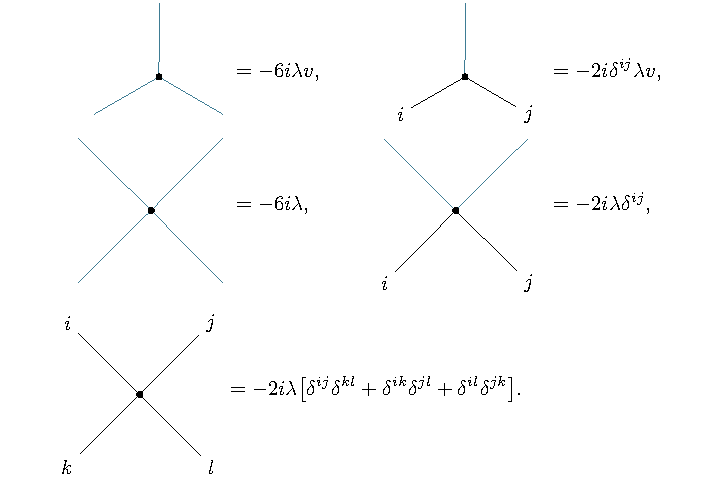
\includegraphics{img/vertex/vertex.pdf}
  \end{center}
  \item Propagators:
  \begin{center}
    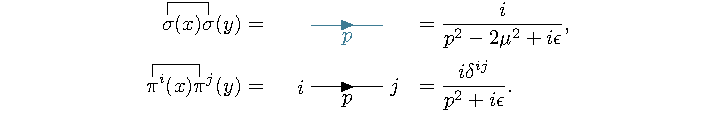
\includegraphics{img/propagator/propagator.pdf}
  \end{center}
\end{itemize}

\plabel{(c)}%
At tree level, $i\mathcal{M}$ has contributions from $s$-channel, $t$-channel, $u$-channel and the single vertex diagram.
\begin{align*}
  i\mathcal{M} &= -4i\lambda \mu^2 \qty[\frac{\delta^{ij}\delta^{kl}}{s - 2\mu^2} + \frac{\delta^{ik}\delta^{jl}}{t - 2\mu^2} + \frac{\delta^{il}\delta^{jk}}{u - 2\mu^2}] \\
  &\phantom{{}={}} - 2i\lambda \qty[\delta^{ij} \delta^{kl} + \delta^{ik}\delta^{jl} + \delta^{il}\delta^{jk}].
\end{align*}
Since $\pi^i$ are massless, at threshold $s=t=u=0$ and therefore $i\mathcal{M} = 0$.
If $N=2$ then $i=j=k=l$ and therefore
\begin{align*}
  i\mathcal{M} &= -2i\lambda \qty[\frac{s}{s - 2\mu^2} + \frac{t}{t - 2\mu^2} + \frac{u}{u - 2\mu^2}] \\
  &= \frac{2i\lambda}{2\mu^2} \qty[s\qty(1+\frac{s}{2\mu^2}+ \cdots) + t\qty(1+\frac{t}{2\mu^2}+\cdots) + u\qty(1+\frac{u}{2\mu^2}+\cdots)] \\
  &= \frac{i\lambda}{\mu^2}\qty[s+t+u + \bigO(p^4)] \\
  &= \bigO(p^4).
\end{align*}
since $s+t+u=0$.

\plabel{(d)}%
The new value that minimize $V$ is given by
\[ (-\mu^2 + \lambda (v^{\mathrm{new}})^2)v^{\mathrm{new}} = a, \]
i.e.
\[ v^{\mathrm{new}} = \sqrt{\frac{\mu^2}{\lambda}} + \frac{a}{2\mu^2} + \bigO(a^2). \]
The new Lagrangian is given by
\begin{align*}
  \mathcal{L}^{\mathrm{new}} &= \frac{1}{2}(\partial_\mu \sigma)^2 - \frac{1}{2}\qty(3\lambda (v^{\mathrm{new}})^2 - \mu^2)\sigma^2 \\
  &\phantom{{}={}} + \qty(\frac{1}{2} \sum_k (\partial_\mu \pi^k)^2) - \frac{1}{2}\qty(\lambda(v^{\mathrm{new}})^2 - \mu^2)\qty(\sum_k (\pi^k)^2) \\
  &\phantom{{}={}} - \lambda v^{\mathrm{new}}\sigma^3 - \qty(\sum_k \lambda v^{\mathrm{new}} (\pi^k)^2\sigma) \\
  &\phantom{{}={}} - \frac{\lambda}{4}\sigma^4 - \qty(\sum_k \frac{\lambda}{2} \sigma^2 (\pi^k)^2) - \qty(\sum_k \frac{\lambda}{4}(\pi^k)^2)^2.
\end{align*}
The $\pi^i$ particles have acquired a mass
\[ m_\pi^2 = \lambda(v^{\mathrm{new}})^2 - \mu^2 = \frac{a}{v^{\mathrm{new}}} \approx \frac{a}{v} = \frac{a\sqrt{\lambda}}{\mu}. \]
The Feynman rules above for vertices still apply after replacing $v$ with $v^{\mathrm{new}}$.
Therefore
\begin{align*}
  i\mathcal{M} &= -4i\lambda \mu^2 \qty(\frac{v^{\mathrm{new}}}{v})^2 \qty[\frac{\delta^{ij}\delta^{kl}}{s - 2\mu^2} + \frac{\delta^{ik}\delta^{jl}}{t - 2\mu^2} + \frac{\delta^{il}\delta^{jk}}{u - 2\mu^2}] \\
  &\phantom{{}={}} - 2i\lambda \qty[\delta^{ij} \delta^{kl} + \delta^{ik}\delta^{jl} + \delta^{il}\delta^{jk}].
\end{align*}
At threshold $t = u = 0$ and therefore
\begin{align*}
  i\mathcal{M} &= - 2i\lambda \delta^{ij} \delta^{kl} \frac{(v^{\mathrm{new}}/v)^2 - 1 + s/(2\mu^2)}{s/(2\mu^2) - 1} \\
  &= - 2i\lambda \delta^{ij} \delta^{kl} \frac{3m_\pi^2}{2m_\pi^2 - \mu^2} \\
  &\approx 6i \delta^{ij} \delta^{kl} \frac{a}{v^3}.
\end{align*}

\prule

\plabel{2 (a)}%
The Feynman rules are given below.
\begin{itemize}
  \item Vertices:
  \begin{center}
    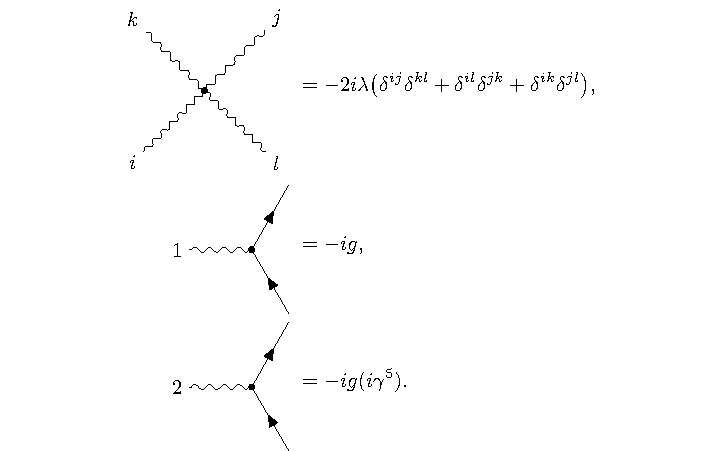
\includegraphics{img/yukawa/unbroken/vertex/vertex.pdf}
  \end{center}
  \item Propagators:
  \begin{center}
    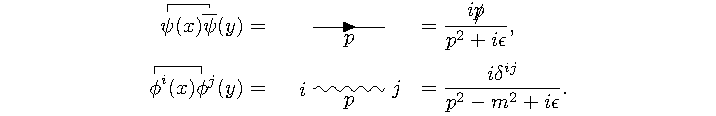
\includegraphics{img/yukawa/unbroken/propagator/propagator.pdf}
  \end{center}
\end{itemize}
Since $\psi$ is massless, the only decay is $\phi^i \rightarrow \overline{\psi}+\psi$, which could happen as long as $m > 0$ and $g > 0$.

\plabel{(b)}%
The conserved current corresponding to $\psi \rightarrow e^{i\alpha} \psi$ is
\[ j^\mu = \overline{\psi} \gamma^\mu \psi, \]
where the charge is the particle number of $\psi$.
\par
Since
\[ g\overline{\psi}(\phi^1 + i\gamma^5 \phi^2) \psi = g\qty[\psi_{\mathrm{L}}^\dagger \psi^{\vphantom{\dagger}}_{\mathrm{R}} (\phi^1 + i\phi^2) + \qty(\psi_{\mathrm{L}}^\dagger \psi^{\vphantom{\dagger}}_{\mathrm{R}} (\phi^1 + i\phi^2))^\dagger], \]
the action is invariant under $\psi \rightarrow e^{i\alpha \gamma^5} \psi$ and $(\phi^1 + i\phi^2) \rightarrow e^{-2i\alpha} (\phi^1 + i\phi^2)$.
The conserved current is given by
\[ j^\mu = 2(\phi^1 \partial^\mu \phi^2 - \phi^2 \partial^\mu \phi^1) + \overline{\psi}\gamma^\mu \gamma^5 \psi. \]
The charge is the total particle number of the complex field $\phi^1 + i\phi^2$ plus the number of right-handed $\psi_{\mathrm{R}}$ minus left-handed $\psi_{\mathrm{L}}$.
\par
The symmetries corresponding to spacetime rotation and translation are the angular momentum and energy-momentum tensor, respectively.

\plabel{(c)}%
The rotation symmetry $\psi \rightarrow e^{i\alpha \gamma^5} \psi$ and $(\phi^1 + i\phi^2) \rightarrow e^{-2i\alpha} (\phi^1 + i\phi^2)$ is broken.
Since $v^2 = \mu^2 / \lambda$, the Lagrangian is given by (removing constant terms)
\begin{align*}
  \mathcal{L} &= \frac{1}{2}(\partial_\mu \sigma)^2 - \frac{1}{2}(2\mu^2)\sigma^2 + \frac{1}{2}(\partial_\mu \pi)^2 + \overline{\psi}\qty(i\slashed{\partial} - \frac{g\mu}{\sqrt{\lambda}}) \psi \\
  &\phantom{{}={}} - \sqrt{\lambda}\mu\sigma^3 - \sqrt{\lambda}\mu\sigma \pi^2 - \frac{\lambda}{4}\sigma^4 - \frac{\lambda}{2} \sigma^2 \pi^2 - \frac{\lambda}{4}\pi^4 - g\overline{\psi}(\sigma + i\gamma^5 \pi) \psi.
\end{align*}
The Feynman rules are listed below.
\begin{itemize}
  \item Propagators:
  \begin{center}
    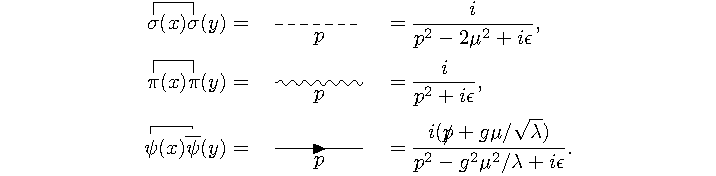
\includegraphics{img/yukawa/broken/propagator/propagator.pdf}
  \end{center}
  \item Vertices:
  \begin{center}
    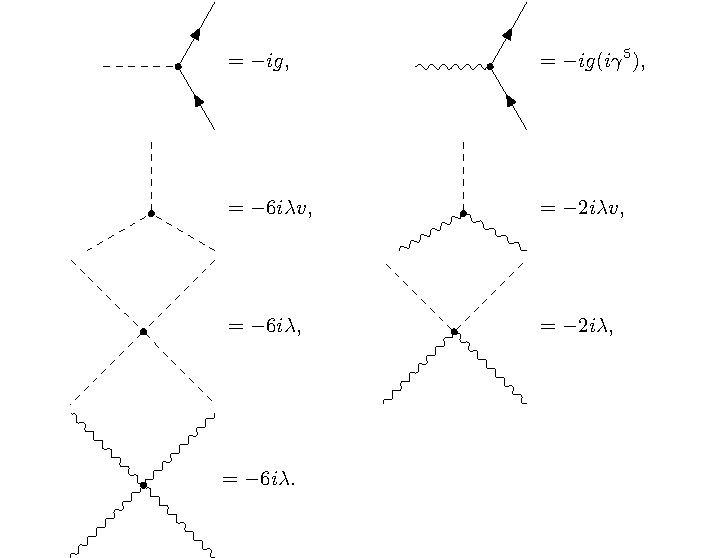
\includegraphics{img/yukawa/broken/vertex/vertex.pdf}
  \end{center}
\end{itemize}
The symmetry reduces to $\psi \rightarrow e^{i\alpha}\psi$ only and yields $j^\mu = \overline{\psi}\gamma^\mu \psi$.

\plabel{(d)}%
The fermion mass is $m_\psi = g\mu/\sqrt{\lambda}$.
If $g\ll \sqrt{\lambda}$ then $m_\psi\ll \mu$.
The decays are given by
\begin{align*}
  \abs{\mathcal{M}(\sigma \rightarrow \overline{\psi}\psi)}^2 &= g^2 \sum_{r,s} \overline{v}^r(\mu/\sqrt{2},-\vb{p}) u^s(\mu/\sqrt{2},\vb{p})\overline{u}^s(\mu/\sqrt{2},\vb{p}) v^r(\mu/\sqrt{2},-\vb{p}) \\
  &= 8g^2 \abs{\vb{p}}^2, \\
  \Gamma(\sigma \rightarrow \overline{\psi}\psi) &= \frac{g^2}{8\pi (2\mu^2)}\qty(2\mu^2 - 4\frac{g^2 \mu^2}{\lambda})^{3/2} \approx \frac{g^2 \sqrt{2\mu^2}}{8\pi},
\end{align*}
and
\begin{align*}
  \abs{\mathcal{M}(\sigma \rightarrow \pi\pi)}^2 &= 4\lambda^2 v^2 = 4\lambda \mu^2, \\
  \Gamma(\sigma \rightarrow \pi\pi) &= \frac{4\lambda \mu^2}{16\pi (2\mu^2)} \frac{\sqrt{2\mu^2}}{2} = \frac{\lambda \sqrt{2\mu^2}}{16\pi}.
\end{align*}
In total
\begin{align*}
  \Gamma &= \frac{(2g^2 + \lambda)\sqrt{2\mu^2}}{16\pi} \approx \frac{\lambda \sqrt{2\mu^2}}{16\pi}, \\
  \tau &= \frac{1}{\Gamma} = \frac{16\pi}{\lambda\sqrt{2\mu^2}}.
\end{align*}

\end{document}
